%!TEX root = ../StrinJet.tex

\section{Simulate with PYTHIA 8 sQCD with CR1 and rope}%
\label{sec:CRorRope}
\begin{figure}[ht]
        \begin{center}
                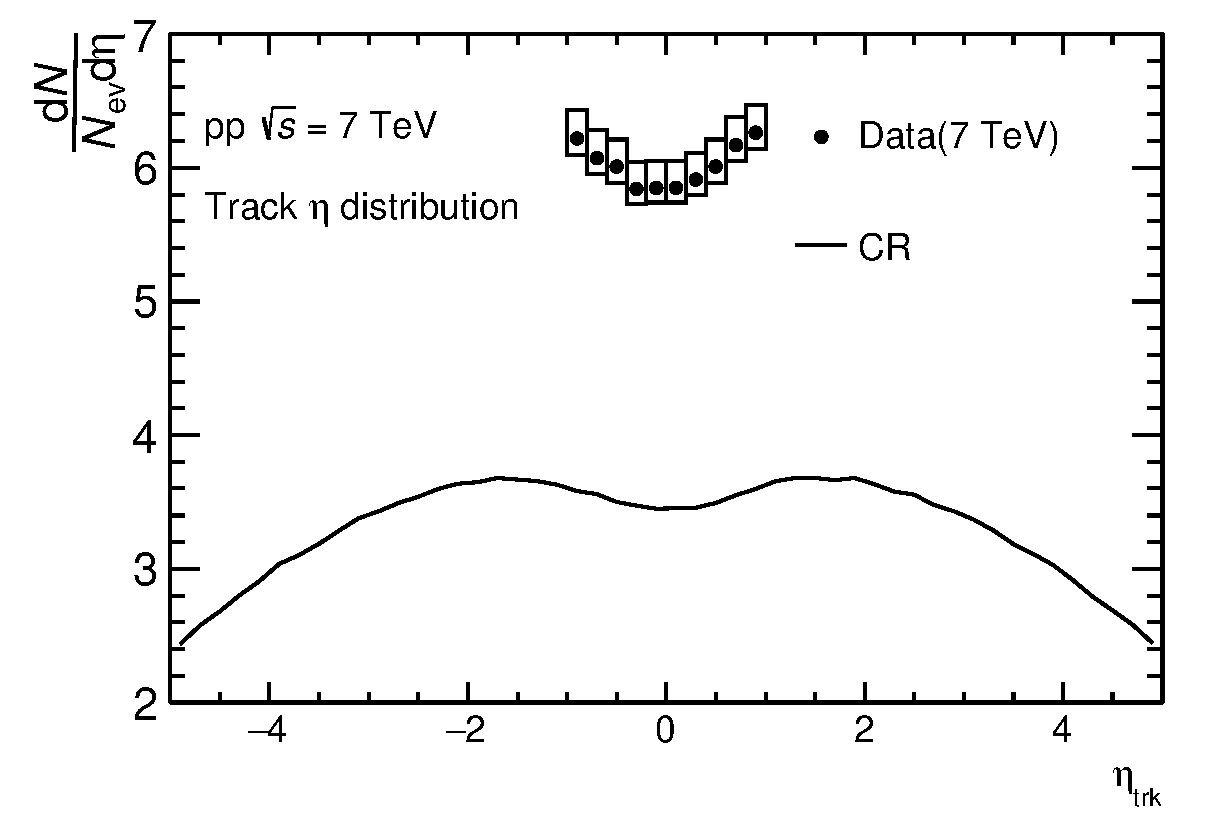
\includegraphics[width=.6\textwidth]{TrkEta}
        \end{center}
        \caption{Track $\eta$ distribution.}
        \label{fig:TrkEta}
\end{figure}


\begin{figure}[ht]
	\begin{center}
		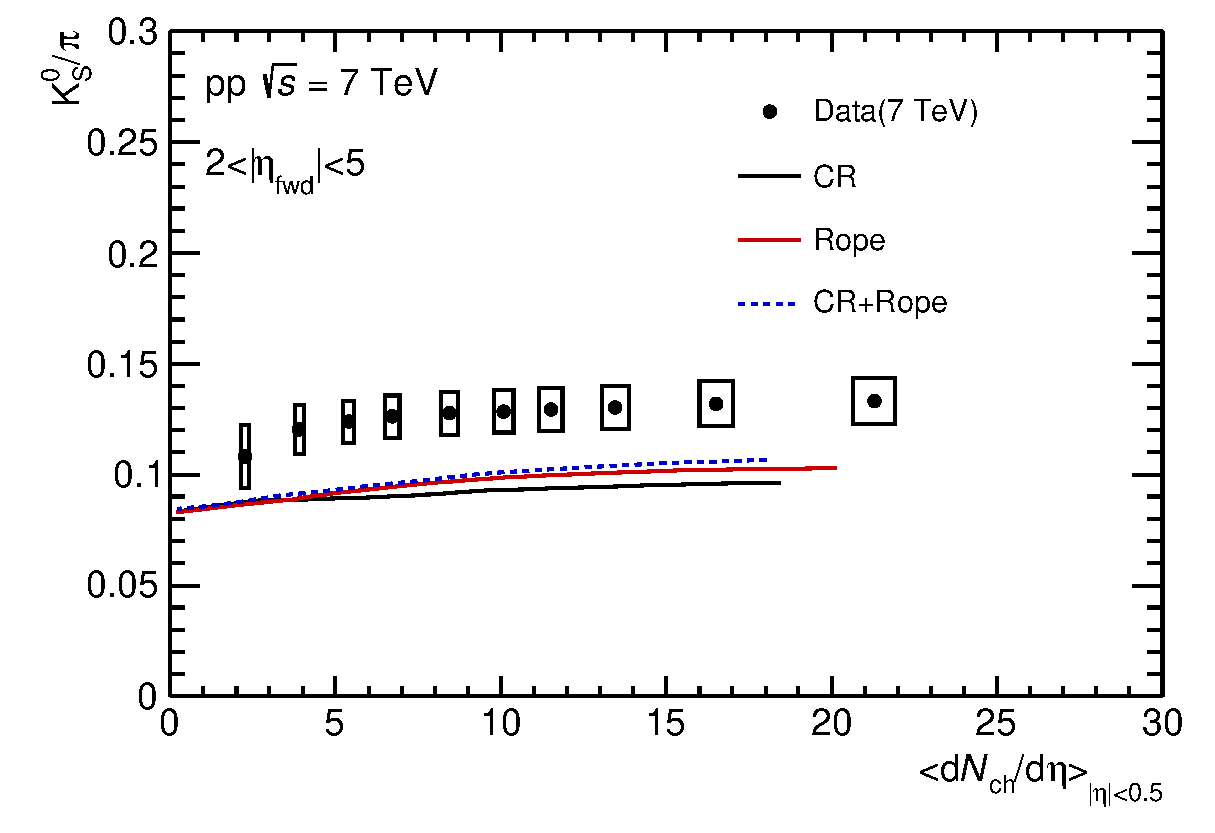
\includegraphics[width=.48\textwidth]{KPiRatio}
		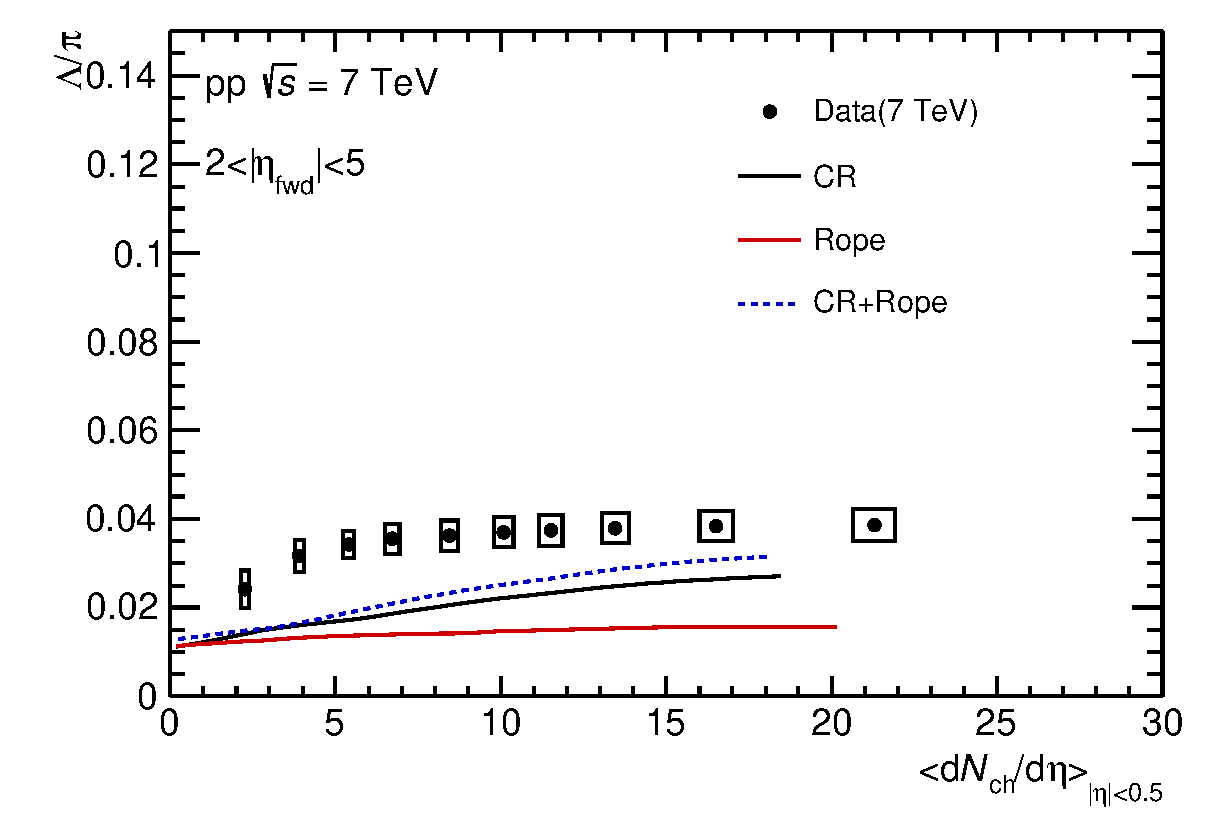
\includegraphics[width=.48\textwidth]{LPiRatio}
		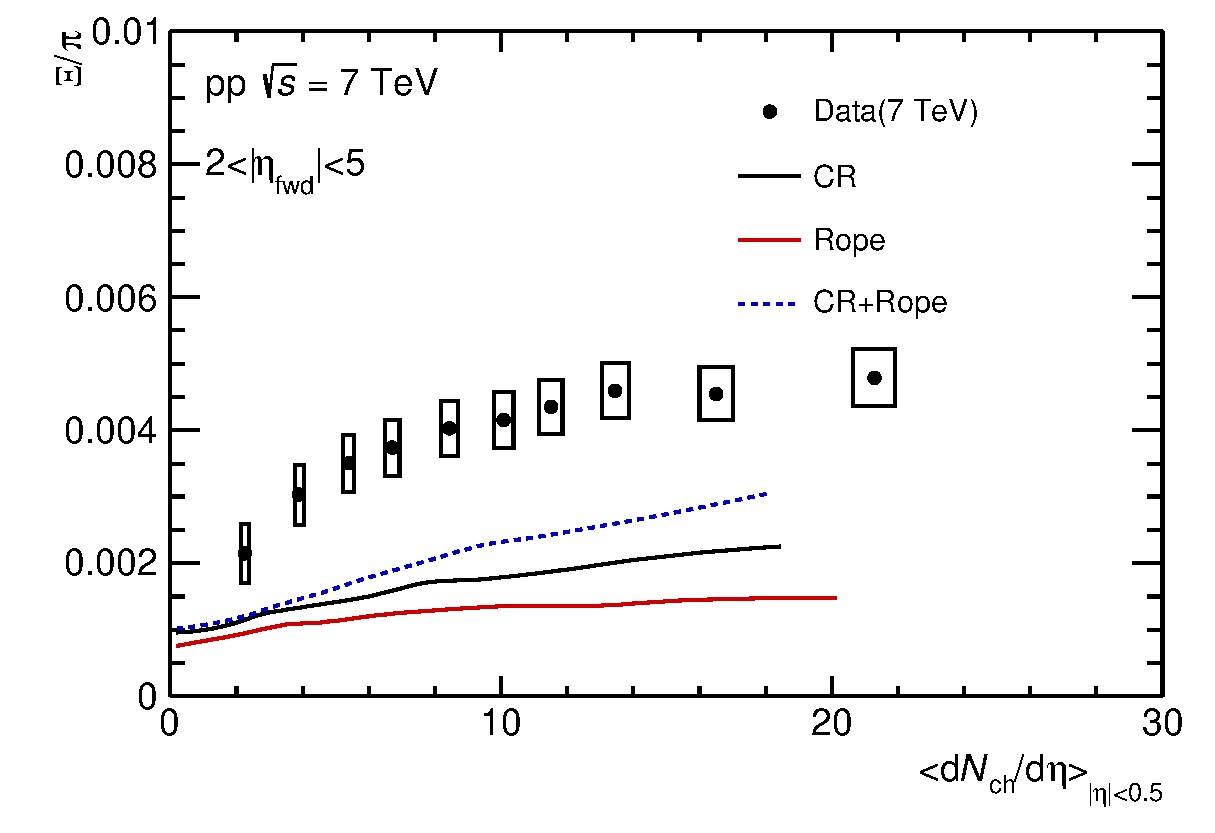
\includegraphics[width=.48\textwidth]{XPiRatio}
		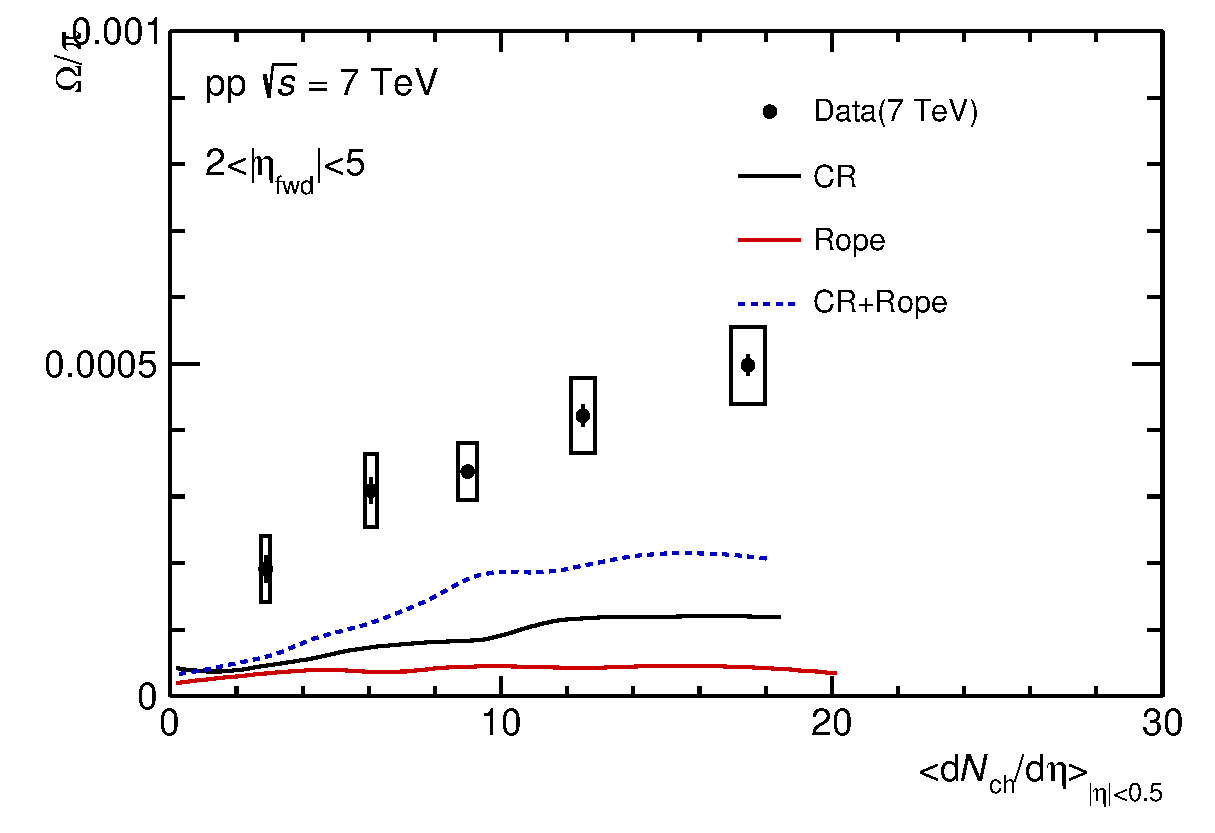
\includegraphics[width=.48\textwidth]{OPiRatio}
	\end{center}
	\caption{Integrated yields ratios of strange particle to $\pi$ with $\dndeta$.}
	\label{fig:IntegralPartoPiRatio}
\end{figure}


\begin{figure}[ht]
        \begin{center}
                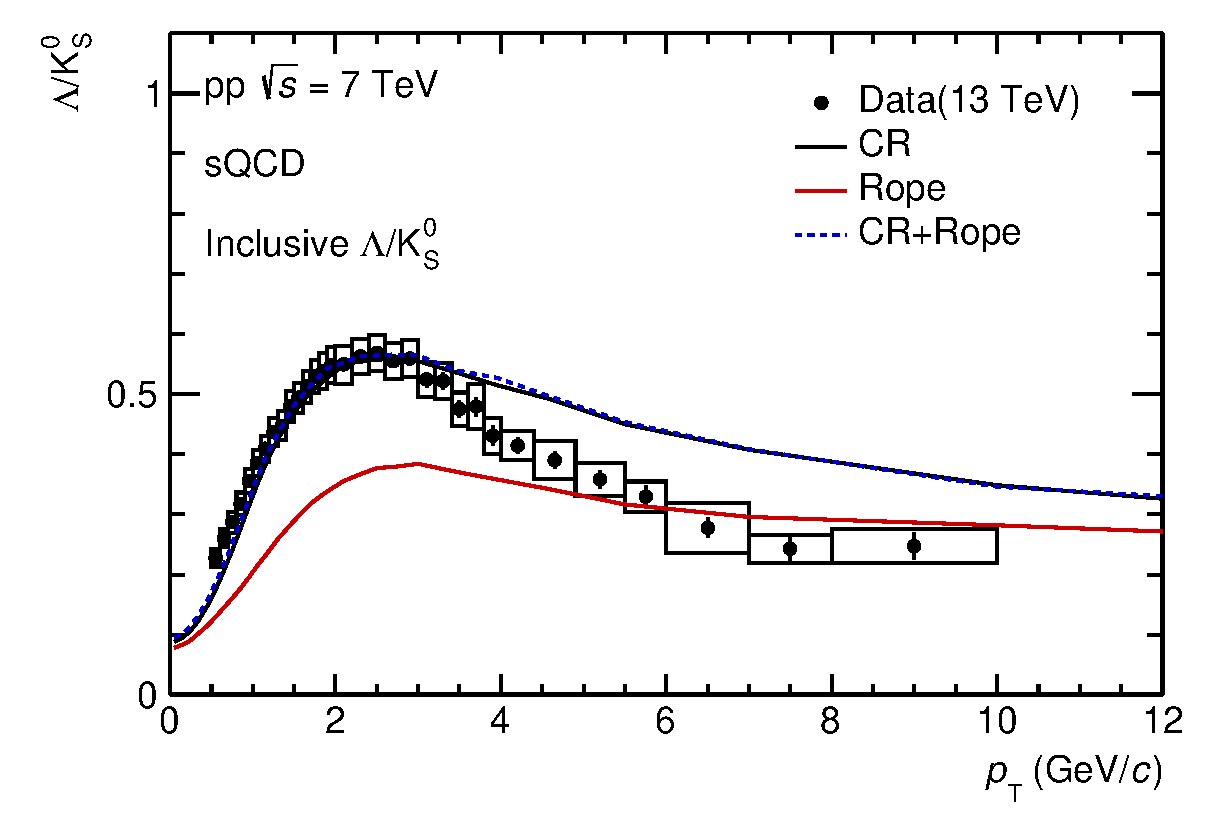
\includegraphics[width=.32\textwidth]{LKRatio_Incl}
                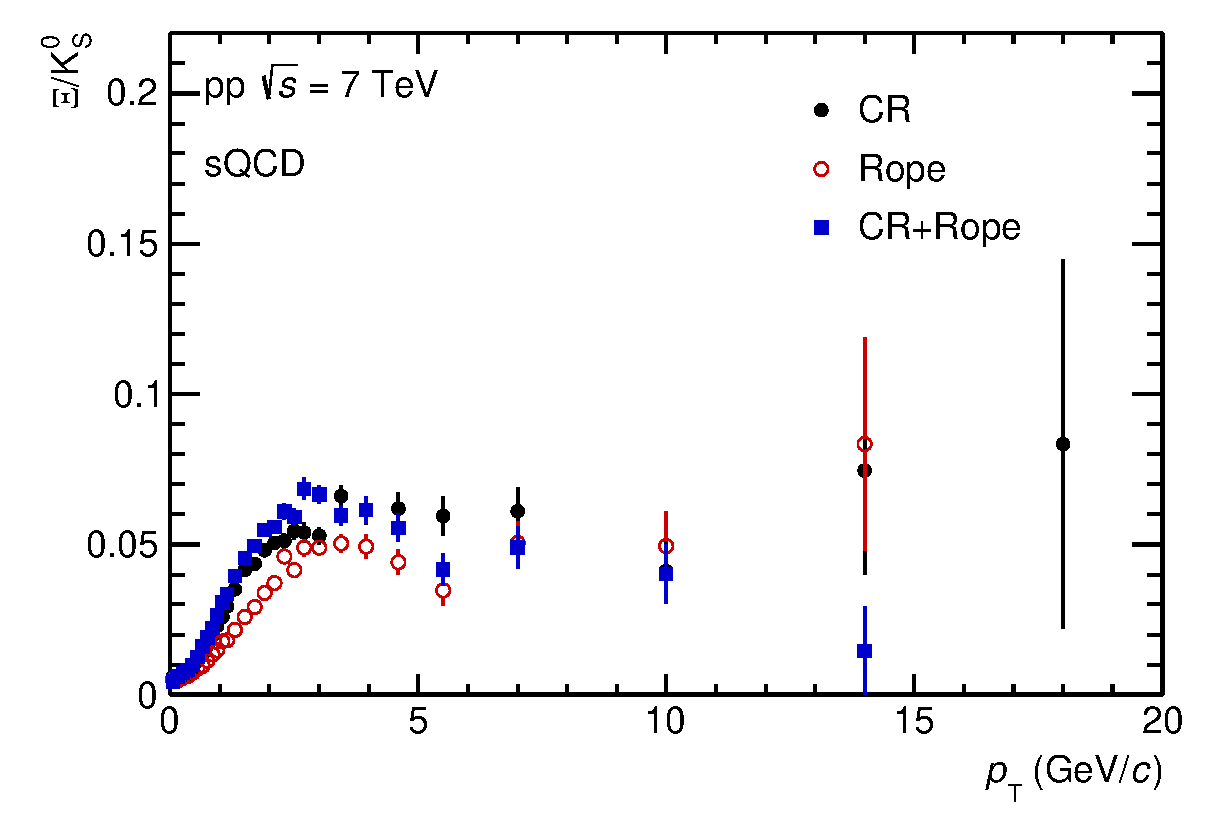
\includegraphics[width=.32\textwidth]{XKRatio_Incl}
                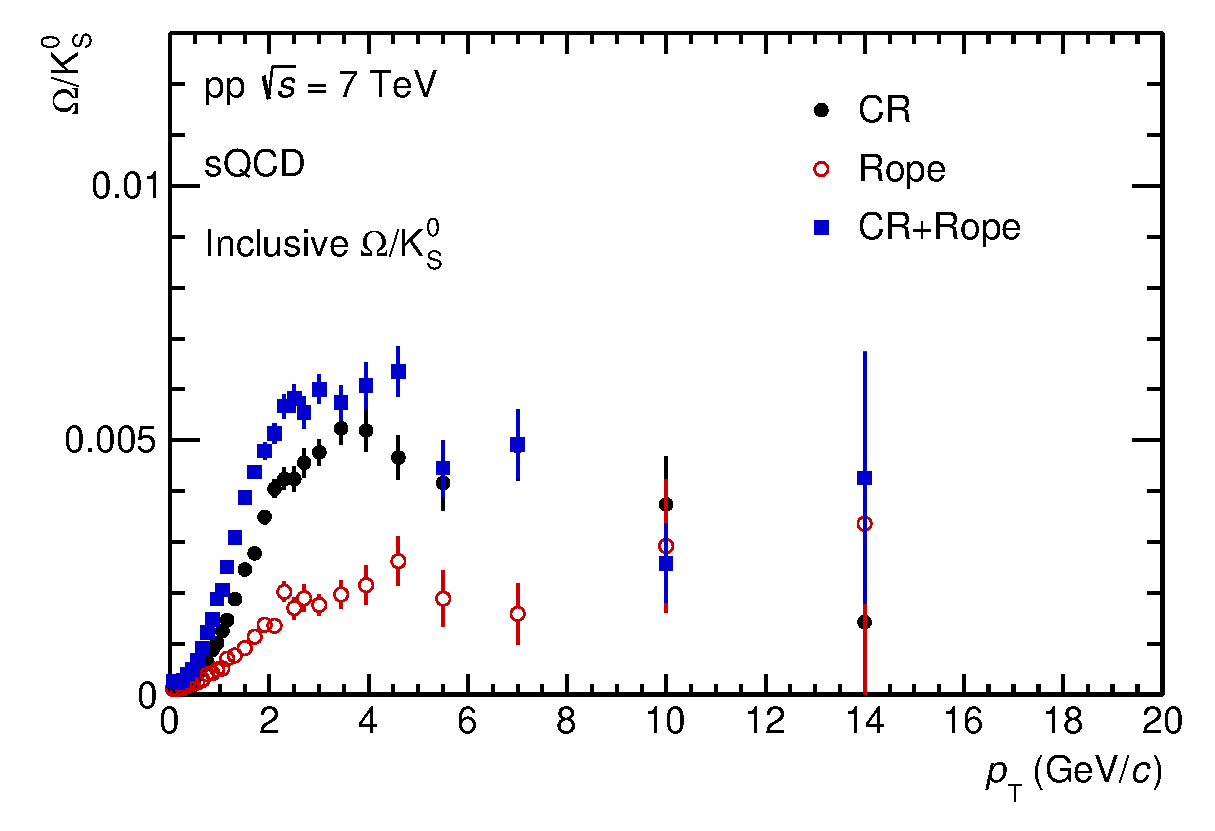
\includegraphics[width=.32\textwidth]{OKRatio_Incl}
                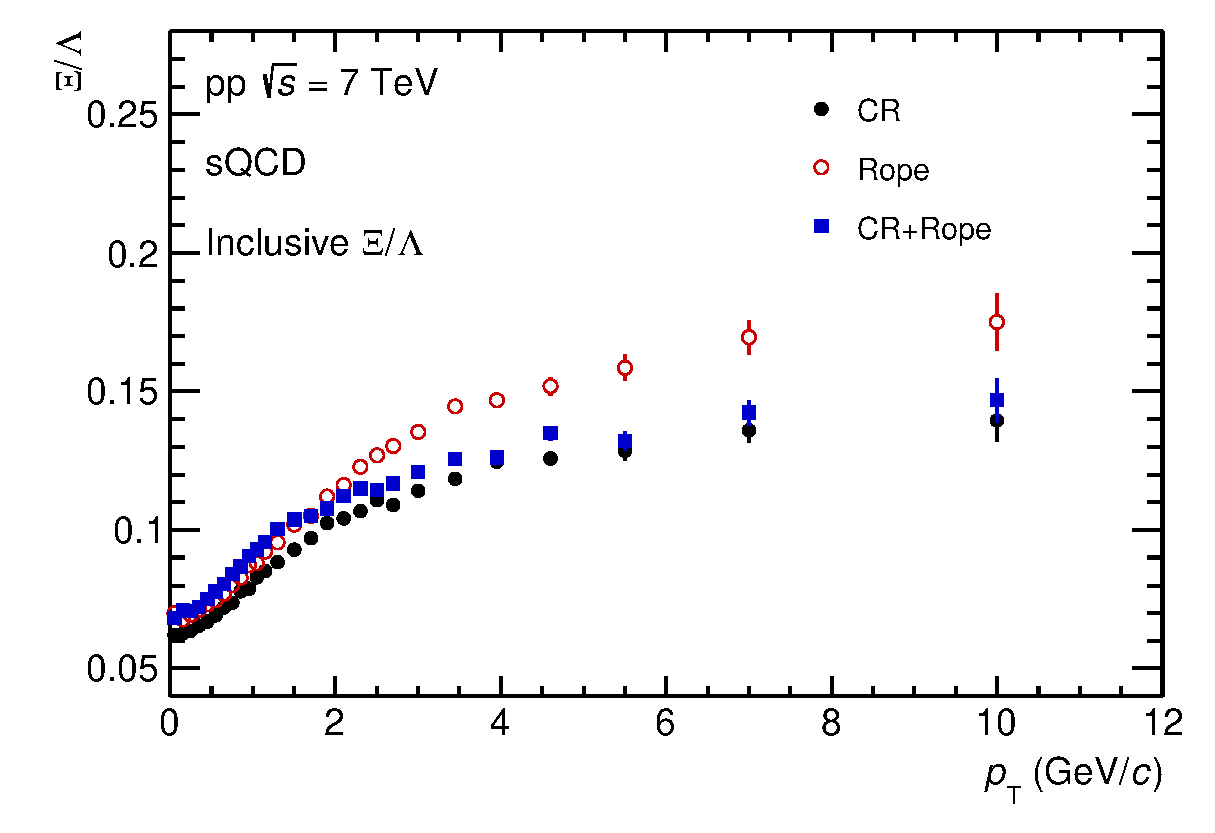
\includegraphics[width=.32\textwidth]{XLRatio_Incl}
                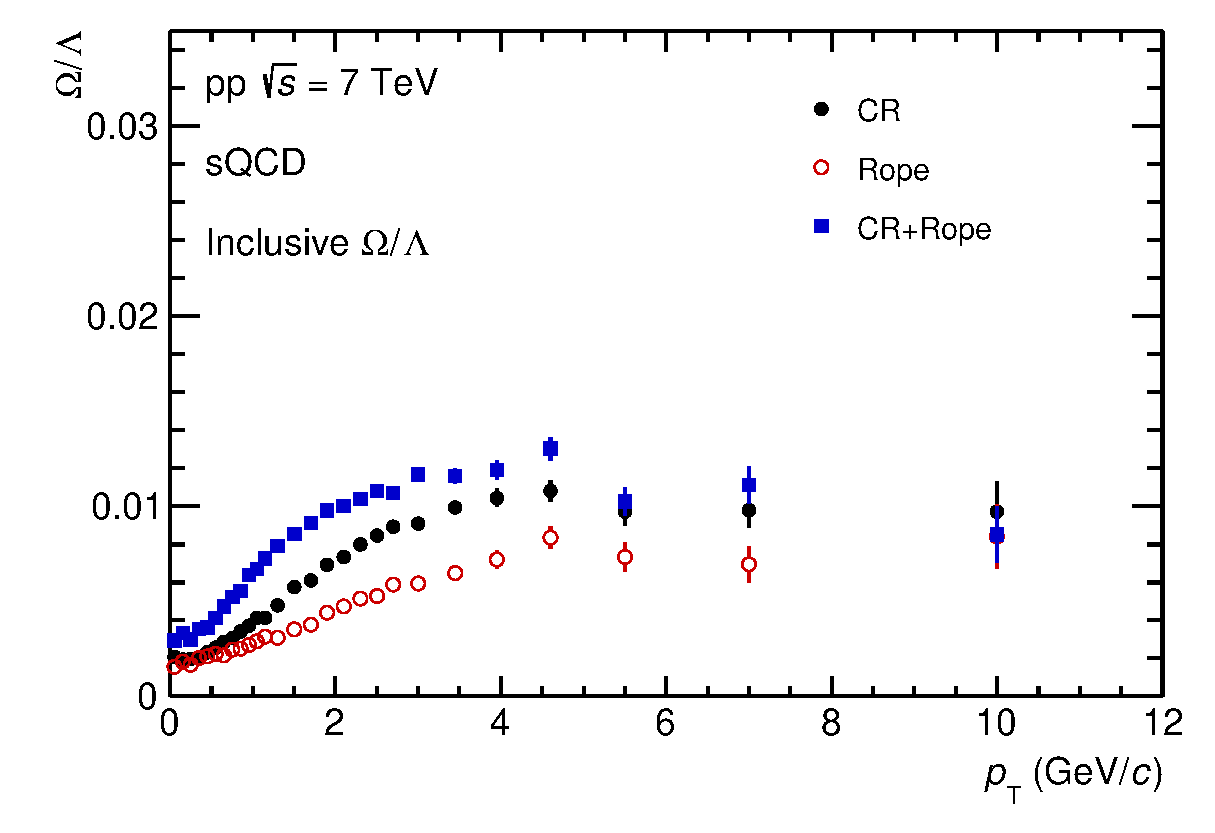
\includegraphics[width=.32\textwidth]{OLRatio_Incl}
                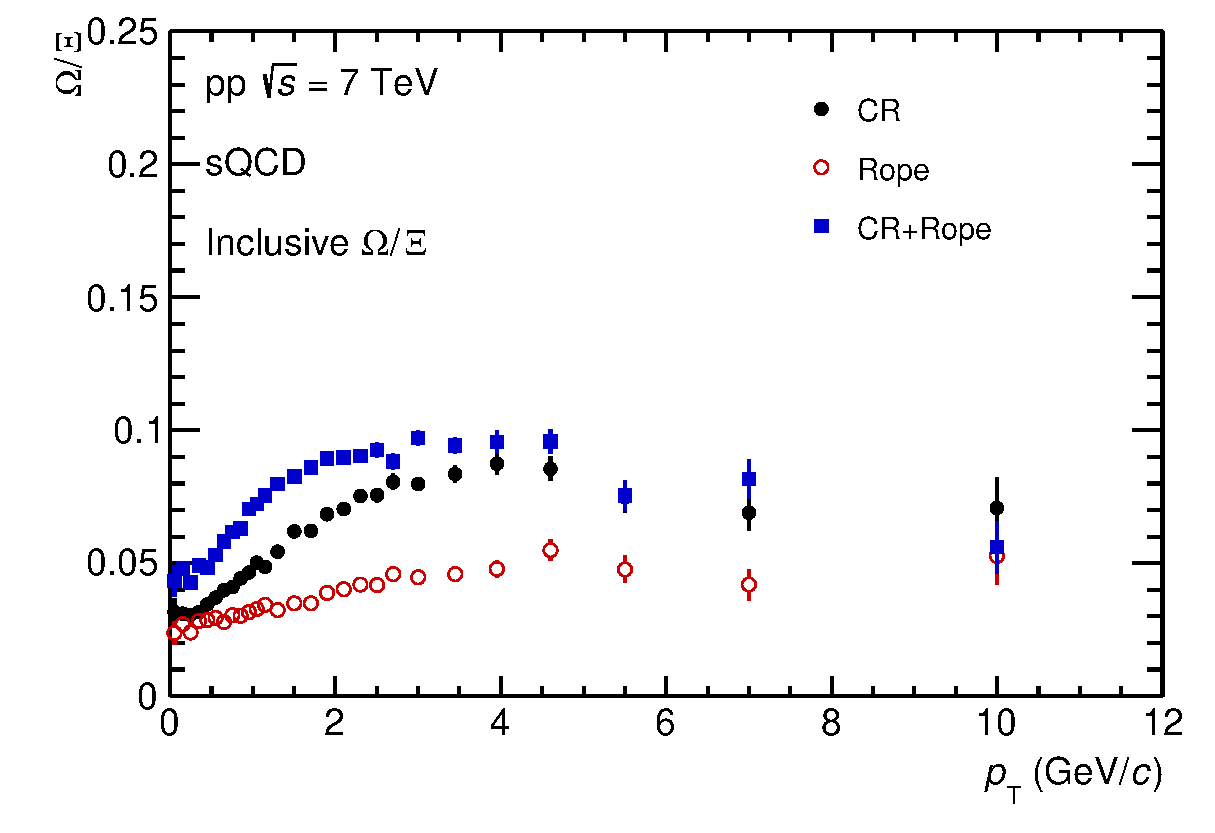
\includegraphics[width=.32\textwidth]{OXRatio_Incl}
        \end{center}
	\caption{Inclusive baryon-to-meson ratio(top) and Baryon-to-meson ratio(bottom) with $\pT$ distribution.}
        \label{fig:InclParRatio}
\end{figure}

\begin{figure}[ht]
        \begin{center}
                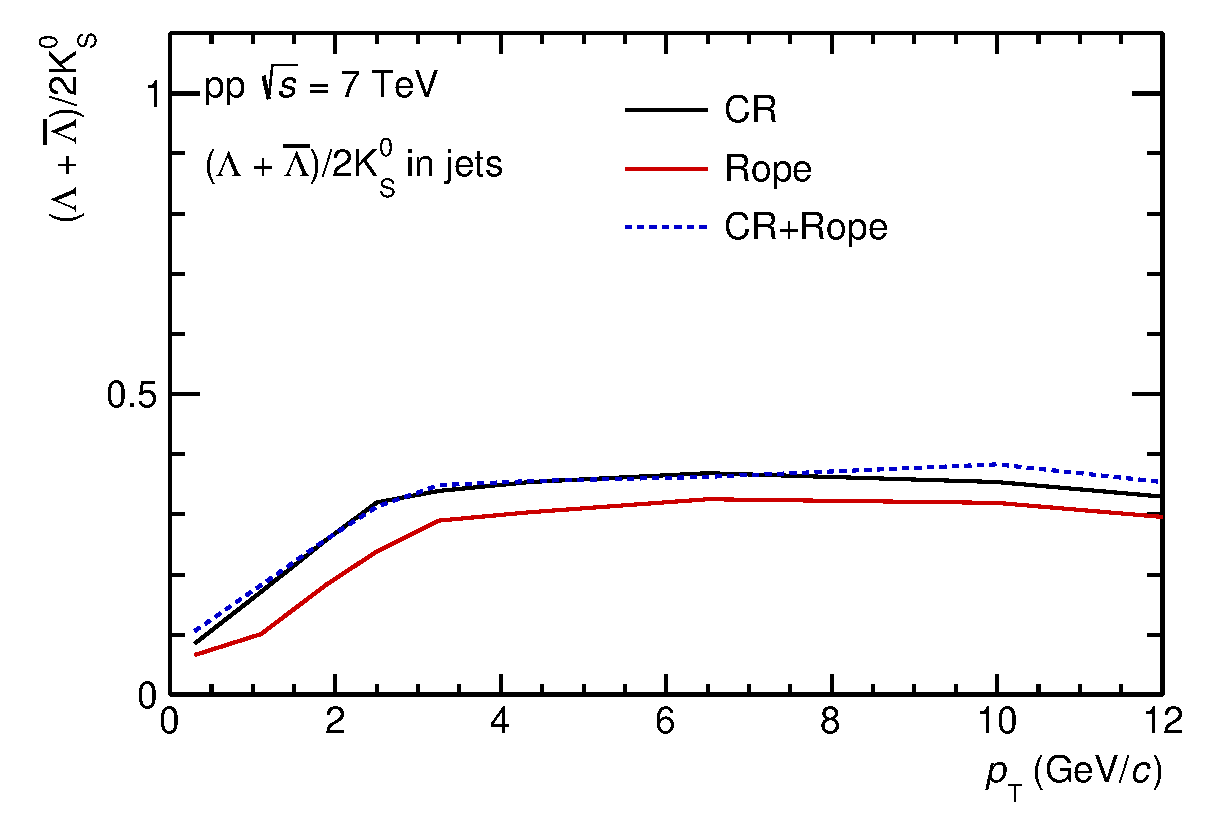
\includegraphics[width=.32\textwidth]{LKRatio_JE}
                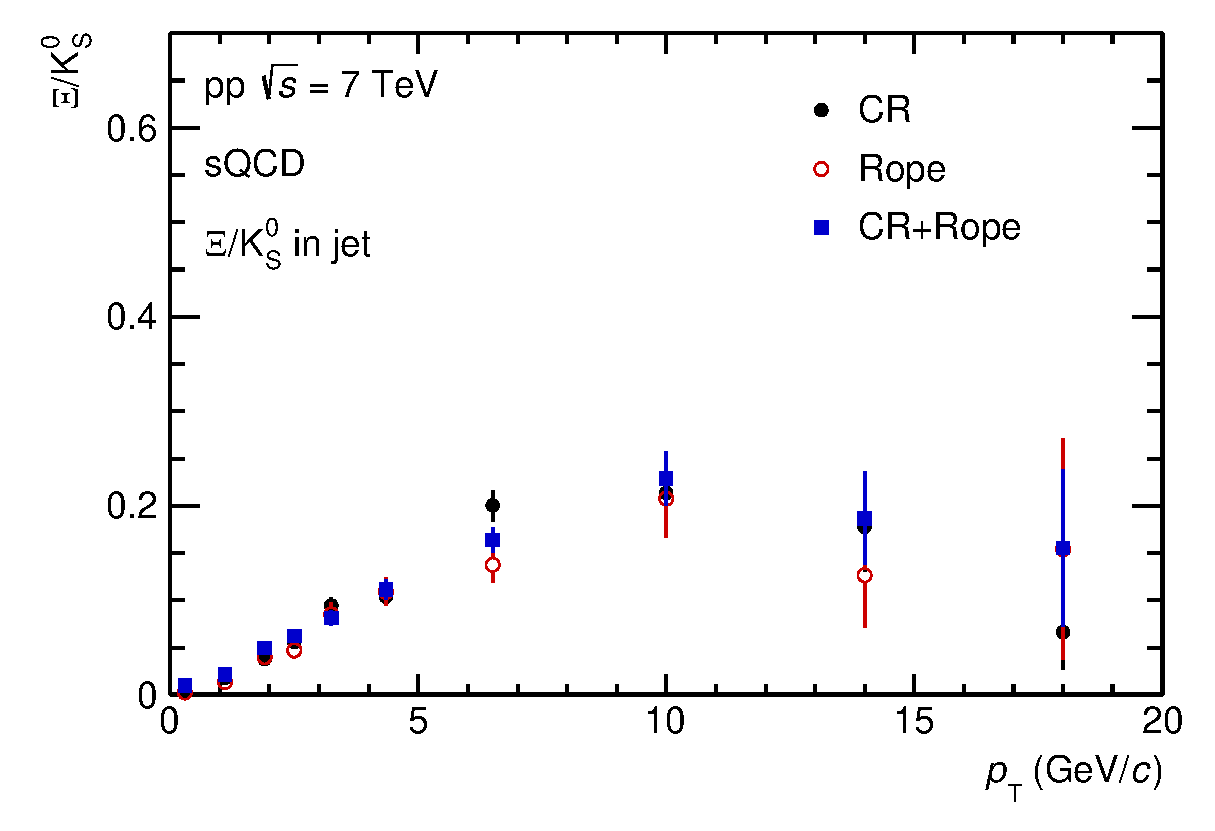
\includegraphics[width=.32\textwidth]{XKRatio_JE}
                \includegraphics[width=.32\textwidth]{OKRatio_JE}
                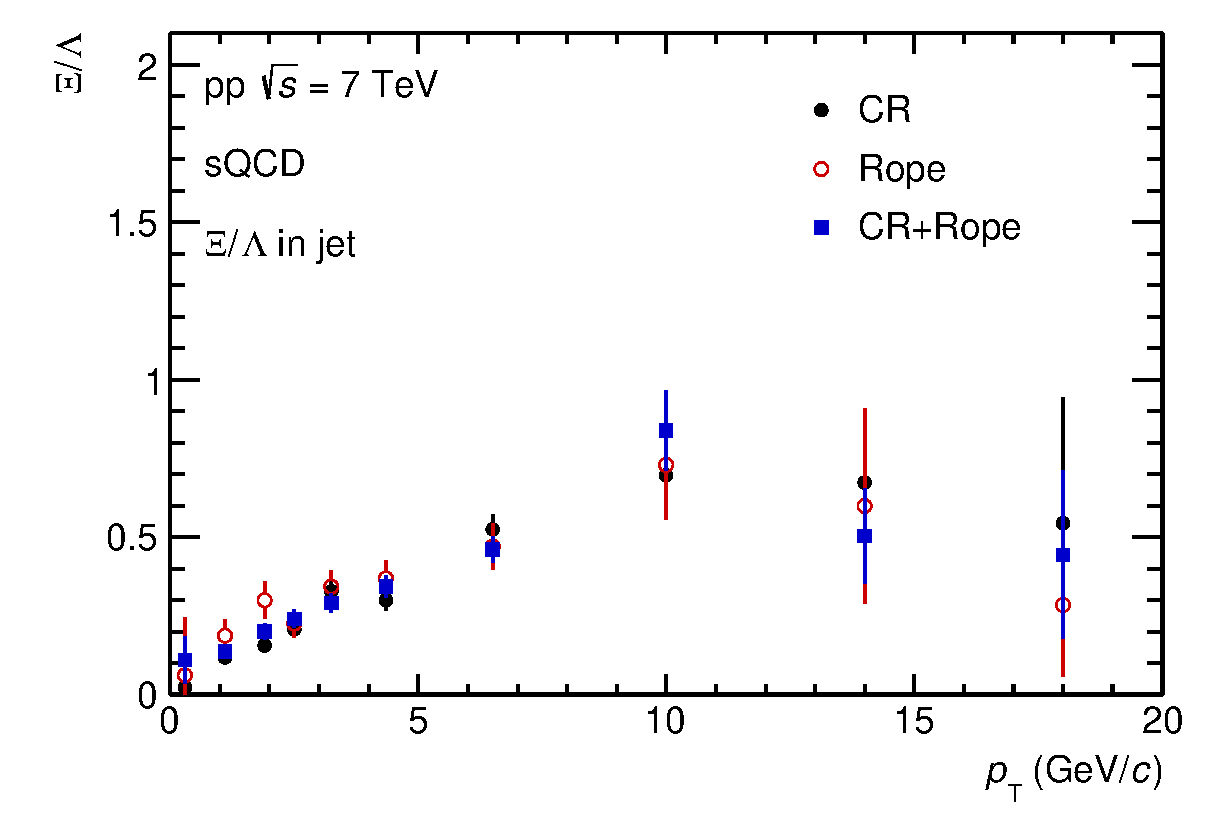
\includegraphics[width=.32\textwidth]{XLRatio_JE}
                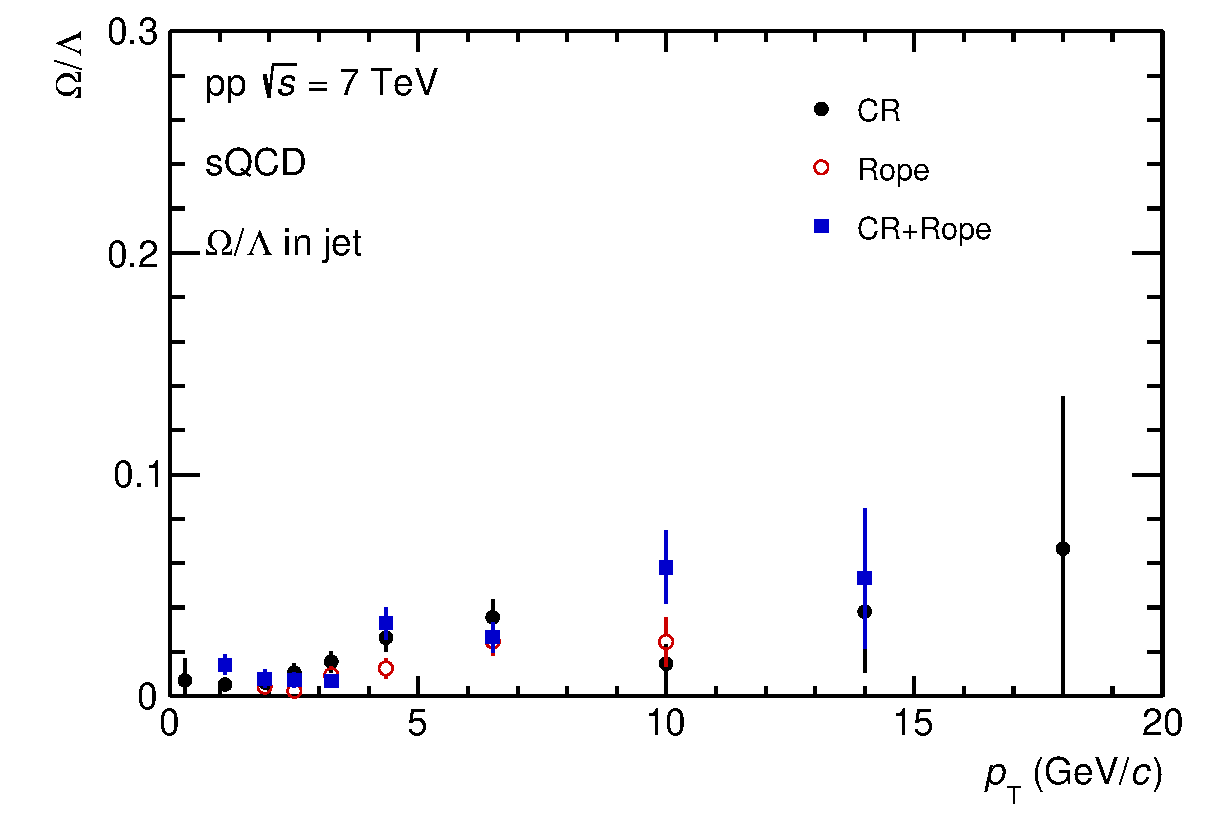
\includegraphics[width=.32\textwidth]{OLRatio_JE}
                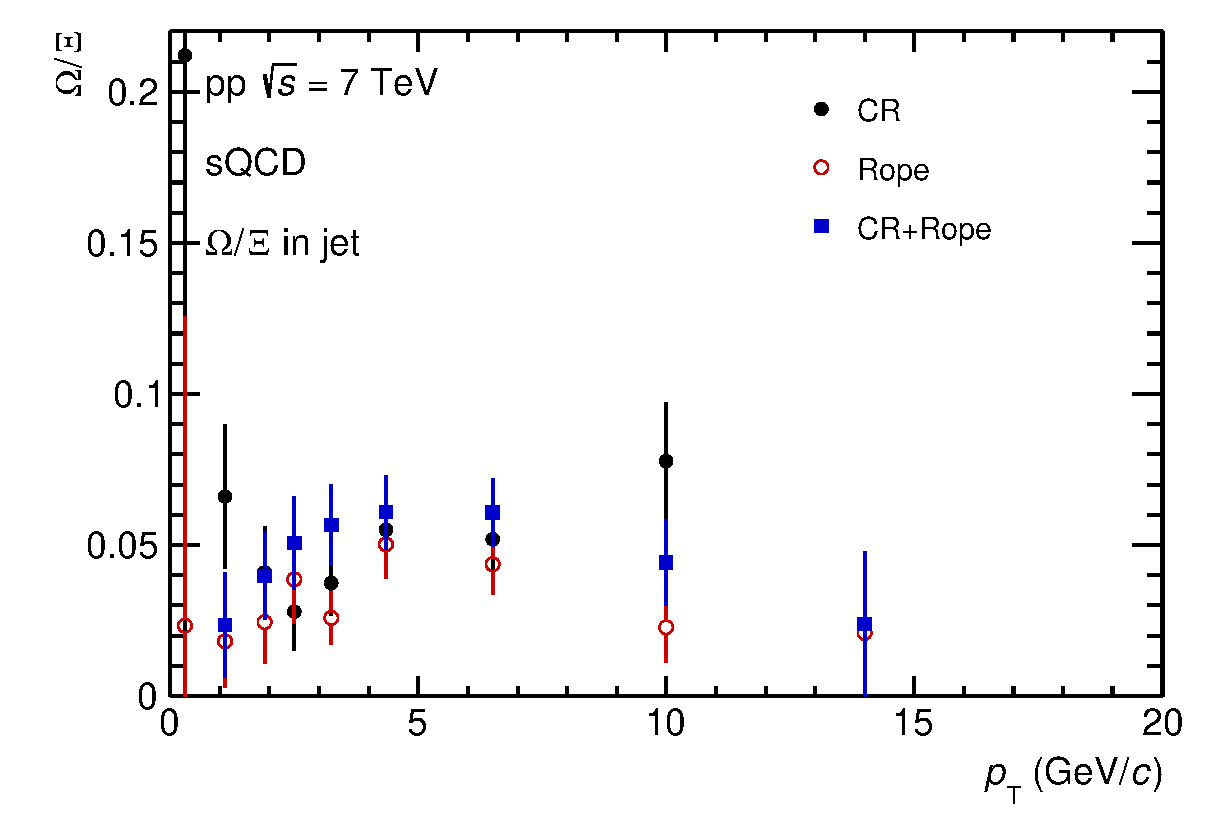
\includegraphics[width=.32\textwidth]{OXRatio_JE}
        \end{center}
        \caption{Baryon-to-meson ratio(top) and Baryon-to-meson ratio(bottom) in jets with $\pT$ distribution.}
        \label{fig:JEParRatio}
\end{figure}

